%% -*- coding: utf-8; -*-

% Use 'digital' option to enable back references. This option is recommended for digital pdf version
%\documentclass[phd,american,digital]{thesispuc}%english thesis
%\documentclass[mscr,american]{thesispuc}%english dissertation
%\documentclass[phd,brazilian]{thesispuc}%tese em portugês
\documentclass[msc,brazilian]{thesispuc}%disseretação em portuguŝ


%%%
%%% Additional Packages
%%%
\usepackage{tabularx}
\usepackage{multirow}
\usepackage{multicol}
\usepackage{colortbl}
\usepackage[%
    dvipsnames,
    svgnames,
    x11names,
    fixpdftex,
    table
]{xcolor}
\usepackage{numprint}
\usepackage{textcomp}
\usepackage{booktabs}
\usepackage{amsmath}
\usepackage{enumitem}
\usepackage{amssymb}

\usepackage{graphicx}
\usepackage{subcaption}
\usepackage{caption}

% ABNT reference style package. The current style is the alphabetical order, if you need
% change to citation order, change in the line above 'alf' to 'num', also at the end replace
% bibliographystyle with the commented version.
\usepackage[alf,bibjustif,abnt-emphasize=bf]{abntex2cite}
%\usepackage{tikz}
%\usepackage[linesnumbered, ruled, vlined]{algorithm2e}
%\usepackage{pgfplots,pgfplotstable} 
%\usepackage{array}

%% numprint 
\npthousandsep{.}
\npdecimalsign{,}

%% ThesisPUC option
%\tablesmode{fig} %% [nada, fig, tab ou figtab]
%\algoritmsmode{none} %% [none ou use] %% Default is [use]
%\codesmode{none} %% [none ou use] %% Default is [use]
%\abreviationsmode{none} %% [none ou use] %% Default is [use]

% \makeatletter  \renewcommand\@biblabel[1]{#1}  \makeatother

%%%
%%% Counters
%%%

%% uncomment and change for other depth values
\setcounter{tocdepth}{1}
%\setcounter{lofdepth}{3}
%\setcounter{lotdepth}{3}
%\setcounter{secnumdepth}{3}

%%%
%%% Misc.
%%%

\usecolour{true}


%%%
%%% Titulos
%%%

\author{Marcos Vinicius Araujo Almeida}
\authorR{Araujo Almeida, Marcos Vinicius} % full name

\advisor{Augusto César Espíndola Baffa}{Prof.} %Name LastName
\advisorR{Baffa, Augusto} %LastName, Name
% If the advisor's department is different from author's department, uncomment the next line and type the correct name and acronym of advisor's institution.
%\advisorInst{institution name}{acronym}

%\coadvisor{Otávio da Fonseca Martins Gomes}{Dr.}
%\coadvisorR{da Fonseca Martins Gomes, Otávio}
%\coadvisorInst{Centro de Tecnologia Mineral}{CETEM/MCTI}

\title{Deep Learning para exames médicos de imagem} %title in portuguese

\titleuk{Deep Learning for Medical Imaging Examinations} %title in english

%%\subtitulo{Aqui vai o subtitulo caso precise}

\day{11}
\month{Novembro}
\year{2023}

\city{Rio de Janeiro}
\CDD{004} 
\department{Informática}
\program{\mbox{Engenharia} da \mbox{Computação}}
\school{\mbox{Engenharia} da \mbox{Computação}}
\university{Pontifícia Universidade Católica do Rio de Janeiro}
\uni{PUC-Rio}


%%%
%%% Jury
%%%

\jury{%
  \jurymember{Luís Fernando Teixeira Bicalho}{Prof.}
    {Departamento de Informática}{PUC-Rio}
  \jurymember{Luiz Fernando Bessa Seibel}{Prof.}
    {Departamento de Informática}{PUC-Rio}
}


%%%
%%% Personal Resume
%%%

\resume{%
% If it fit in one line use this command:
\makebox[\textwidth][s]{Graduando em Engenharia da Computação na PUC-Rio.}%
% If not just type your resume without any special command 
}

%%%
%%% Acknowledgment (REMINDER TO SCHOLARSHIP STUDENTS. Do not forget to thank the agencies that supported your work.)
%%%
\acknowledgment{%
\noindent Para meu orientador Augusto Baffa, por conduzir por todos os caminhos e me ajudar a montar essa tese.
\bigskip

\noindent Para minha mãe, que sempre deu todo seu suor e esforço para fornecer a melhor educação possível para mim.
\bigskip

\noindent Para minha madrinha, meia-irmã e todas as outras pessoas que participaram da minha criação, contribuindo para oque eu sou hoje.
\bigskip

\noindent Agradeço a PUC-Rio pela oportunidade de ser bolsista integral.
\bigskip

\noindent Agradeço a todos os amigos que conheci durante esses 5 anos de faculdade pelo suporte e apoio.



}


%%%
%%% Catalog prekeywords
%%%

\catalogprekeywords{%
  \catalogprekey{Informática}%
}

%%%
%%% Keywords - Don't use % at the end of /key dfinition
%%%

\keywords{%
  \key{Aprendizado Profundo}
  \key{Redes Neurais de Convolução}
  \key{Imagens de Exames médicos}
  \key{Pneumonia}
  \key{InceptionV3}
  \key{ResNet50}
  
}

\keywordsuk{%
  \key{Deep Learning}
  \key{Convolution Neural Networks}
  \key{Medical Imaging}
  \key{Pneumonia}
  \key{InceptionV3}
  \key{ResNet50}
}

%%%
%%% Abstract
%%%

\abstract{%
As Redes Neurais Convolucionais (CNNs) representam um avanço significativo no campo de imagens médicas, redefinindo os métodos de diagnóstico e análise. Sua eficácia se destaca na identificação e classificação de anormalidades, facilitando a detecção precoce de condições como câncer, lesões cerebrais e problemas cardíacos. Nessa tese,  foram comparados modelos baseados em CNNs para determinar o mais eficiente na tarefa de classificar imagens de raio-X pulmonares, com o objetivo de diagnosticar a presença ou ausência de pneumonia. Este trabalho destacou o potencial das CNNs em aplicações práticas, evidenciando sua relevância e eficácia no diagnóstico médico por imagem.
}

\abstractuk{%
Convolutional Neural Networks (CNNs) represent a significant advancement in the field of medical imaging, redefining diagnostic and analytical methods. Their effectiveness is particularly notable in the identification and classification of abnormalities, promoting the early detection of conditions such as cancer, brain injuries, and cardiac issues. In this thesis, CNN-based models were compared to decide the most efficient one for the task of classifying pulmonary X-ray images, aimed at diagnosing the presence or absence of pneumonia. This work highlighted the potential of CNNs in practical applications, underscoring their relevance and efficacy in image-based medical diagnosis.
}

%%%
%%% Dedication
%%%

\dedication{%
Para a minha mãe e minha madrinha, pelo seu suporte e encorajamento.
}

%%%
%%% Epigraph
%%%

%\epigraph{%
%  Not all those who wander are lost
%}
%\epigraphauthor{ J.R.R. Tolkien}
%\epigraphbook{The Fellowship of the Ring}

\epigraph{%
  Nah, I'd win.
}
\epigraphauthor{Satoru Gojo}
\epigraphbook{Jujutsu Kaisen}





\begin{document}
  % -*- coding: utf-8; -*-

\chapter{Introdução}
\label{cha:Introdução}

A cada dia que passa percebemos cada vez mais os impactos da tecnologia no nosso cotidiano, sendo eles positivos ou negativos. Desde inteligências artificiais, que podem nos dar respostas à perguntas simples \cite{Haque_2023}, economizando nosso tempo de pesquisa, até \textit{cyber-ataques} que podem contribuir para o vazamento de dados sensíveis de milhões de pessoas \cite{10.11648/j.epes.20221106.12}.

A Inteligência Artificial, uma área emergente e cada vez mais robusta na tecnologia, simula o conhecimento humano através de máquinas, destacando-se na otimização de processos e no incremento da produtividade. Deep Learing é uma subárea do aprendizado de máquina (\textit{Machine Learning}), que por sua vez é uma subárea da IA. Ela é capaz realizar tarefas relativamente mais complexas como reconhecimento e análise de imagens, reconhecimento de voz e linguagem natural. De acordo com o estudo da PwC foi previsto que até 2030 a Inteligência Artificial pode contribuir em até \$15.7 trilhões para a economia global.\cite{PWC1}

Seguindo por essa lógica, muito entusiastas realizaram diversos projetos para aplicar essas soluções inovadoras na área da saúde. Segundo a empresa de consultoria americana, \textit{Accenture}, até 2026, os Estados Unidos irão economizar US\$ 150 bilhões por ano com cuidados com a saúde por consequência da aplicações de IA.\cite{IST1} Dito isso, será mostrado nesse relátorio, um exemplo de aplicação da Inteligência artificial na área da saúde e possíveis melhoras para criação e enriquecimento de modelos de aprendizado de máquina.


%Falar do doc da OMS sobre os avanços da IA
% https://www.who.int/publications/i/item/9789240029200

\nocite{7422082}
\nocite{7404285}
\nocite{doi:10.1148/ryai.2019180015}
\nocite{7950512}
\nocite{doi:10.1080/21681163.2015.1124249}
\nocite{Hesamian_Jia_He_Kennedy_2019}
\nocite{Gao_Han_Li_Ji_Zhang_Sun_2018}
\nocite{7412749}
\nocite{7501527}
\nocite{6975210}
\nocite{7590963}
\nocite{AREVALO2016248}
\nocite{7426413}
\nocite{pmlr-v136-phillips20a}
\nocite{rajpurkar2017chexnet}
\nocite{7801947}
\nocite{7545996}
\nocite{SUN20174}
\nocite{10.1007/978-3-319-10590-1_53}
 
  % -*- coding: utf-8; -*-

\chapter{Situação Atual}

\label{cha:Situação Atual}

A inteligência artificial na medicina consiste no uso de algoritmos de aprendizado de máquina, aliado com grandes bases de dados, para promover análises mais precisas de exames e melhorar a experiência dos pacientes. Muitos desses modelos de aprendizado fornecem suporte para várias partes do mundo, tanto dentro de hospitais ajuando médicos a tomarem melhores decisões, como também em pesquisas de novos fármacos.

Primeiramente, podemos perceber uma frente bem relevante na área de desenvolvimento de novos medicamentos. O processo de criação até teste que é realizado hoje é extremamente custoso, podendo levar anos de pesquisa. Segundo o artigo feito por Mathew Chun \cite{HARV1}, com a chegada de novos algorítmos de redes neurais, como NLP, diversas áreas desse ramo foram afetas e estão contribuindo positivamente para o aperfeiçoamento de novos remédios. Melhoras significativas foram notadas na aquisição de melhores alvos de genes para servirem de contrariantes para determinas doença; Predição de propriedades dos fármacos antes mesmo da testagem; Geração de padrões moleculares de remédios, nunca antes vistos.

O uso da IA para detecção de doenças e produção de diagnósticos mais precisos se tornou um alido para diferentes clínicos, contribuindo para o aumento de sua produtividade. Justamente pelo fato de máquinas não terem as mesmas limitações fisícas que um humano normal, uma IA pode coletar dados de pacientes como, batimentos cardíacos, respirações por minuto, informações sobre a pressão, enquanto o médico não estiver presente e notificar quando notar algo fora dos padrões. Como dito no estudo da IBM, um cliente da empresa conseguiu desenvolver um modelo preditivo de inteligência artificial para detectar condições de sepse grave em bebês pré-maturos. \cite{IBM1} %aumentar isso%

A inteligência artificial também pode ser aplicada no exame de imagens médicas. Esse ramo é muito importante na medicina, já que elas são necessárias para a visualização de órgãos internos com o objetivo de detectar anomalias em sua estrutura ou funcionamento. Muitos dispositivos podem ser utilizados, gerando imagens ou vídeos de qualidade, sendo eles, raios-x, tomografias computadorizadas, ressonâncias magnéticas, tomografias por emissão de pósitrons (PET), e ultrassonografias. Após a captura, essas imagens devem ser analisadas e compreendidas para a detecção precisa de anormalidades. Caso seja identificada alguma inconformidade, devem ser apresentadas sua localização exata, tamanho e forma da anomalia. Hoje, sistemas de saúdes mais inteligentes, tem como objetivo aplicar IA para realizar essas tarefas de análise, que antes eram feitas por médicos treinados com sua experiência adquirida ao longo dos anos.


Estudos indicam que o uso de IA's em imagens médicas podem ser tão eficiente quanto um radiologista detectando sinais de câncer de mama em um exame. De acordo com o centro de tecnologia de Massachusetts, foi criado um modelo de aprendizado de máquina capaz de detectar o crescimento de um tumor maligno na mama de uma paciente, 5 anos antes de se formar completamente e deixá-la em condições graves. \cite{MIT1} O modelo foi treinado com dados de mais de 60.000 pacientes e, o mesmo conseguiu detectar padrões sutis no tecido mamário que indicariam futuros casos de tumores na região. 


%https://www.ibm.com/topics/artificial-intelligence-medicine#:~:text=How%20is%20artificial%20intelligence%20used,health%20outcomes%20and%20patient%20experiences.

%%https://www.sbmastologia.com.br/inteligencia-artificial-preve-cancer-de-mama-cinco-anos-antes/ 
  % -*- coding: utf-8; -*-
\chapter{Objetivos}
\label{cha:Objetivos}

Como dito no capítulo anterior, o ramo de imagens médicas é extramente importante para a medicina e aplicar técnicas de inteligência artificial para automatizar o processo de análise, pode ser um ganho extremamente positivo. Portanto, o propósito desta tese é explorar diferentes modelos de inteligência artificial que possam classificar, com base em imagens de raio-X do pulmão, se um indivíduo possui pneumonia. O estudo visa comparar os resultados de diferentes modelos e variações para identificar o mais eficaz entre as opções disponíveis. Para tal, serão empregadas diversas métricas e testes na avaliação desses modelos. 

Em primeiro momento, serão testados diversos tipos de imagens, incluindo exemplos de pulmões saudáveis e outros afetados por pneumonia, como ilustrado nas figuras \ref{subfig:pictures/pneumonia.jpeg} e \ref{subfig:pictures/normal.jpeg}.

\subimages{Exemplos de imagem de entrada}{45}
{
 \subimage[Pulmão afetado por pneumonia]{.45}{pictures/pneumonia.jpeg}
 \subimage[Pulmão saudável]{.45}{pictures/normal.jpeg} \\
}


Após recebidas essas entradas, os modelos devem, de alguma maneira, classificar as imagens em \textbf{NORMAL} ou \textbf{PNEUMONIA}, retornando sua confiança para aquela previsão. Um exemplo de saída pode observado na imagem \ref{pic:resultado_modelo}.

\newpage 

\begin{figure}[!ht]
    \begin{center}
    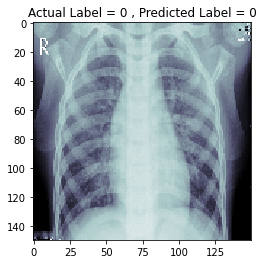
\includegraphics[width=200pt]{pictures/resultado_exemplo.png}
    \caption{Exemplo de resultado do modelo}
    \label{pic:resultado_modelo}
    \end{center}
\end{figure}


Os dados obtidos vêm, por padrão, com um gabarito anexado, o que possibilitou a comparação direta. Contudo, na aplicação prática, o resultado se limitaria à classe prevista pelo modelo.
  % -*- coding: utf-8; -*-

\chapter{Pesquisas Realizadas}
\label{cha:Pesquisas Realizadas}


Nesse capítulo serão abordadas todas as pesquisas realizadas para a confecção dessa tese. Os tópicos variam desde temas mais técnicos explorando diferentes tipos de redes neurais e otimizadores, até assuntos mais voltados para a área médica.




\section{Pneumonia}


A pneumonia é uma infecção que inflama os sacos de ar em um ou ambos os pulmões, onde esses sacos podem se encher de líquido ou pus, provocando tosse com pus ou muco, febre, calafrios e dificuldade para respirar, podendo ser melhor representado na imagem \ref{pic:pneumonia}. A condição pode ser causada por uma variedade de organismos, incluindo bactérias, vírus e fungos. A gravidade da pneumonia pode variar de leve a grave, sendo mais perigosa para bebês e crianças pequenas, pessoas com mais de 65 anos e pessoas com problemas de saúde ou sistemas imunológicos enfraquecidos \cite{WHO2023Pneumonia}. Podemos confirmar esses detalhes também na imagem \ref{pic:stats_pneumonia}, onde observamos que em todas as condições as pessoas mais afetas por pneumonia são idosas. Essa imagem retrata um estudo feito da incidência de casos de pneumonia nos EUA dos anos de 2007 até 2010 \cite{doi:10.2147/COPD.S140378}.

\begin{figure}[!ht]
    \begin{center}
    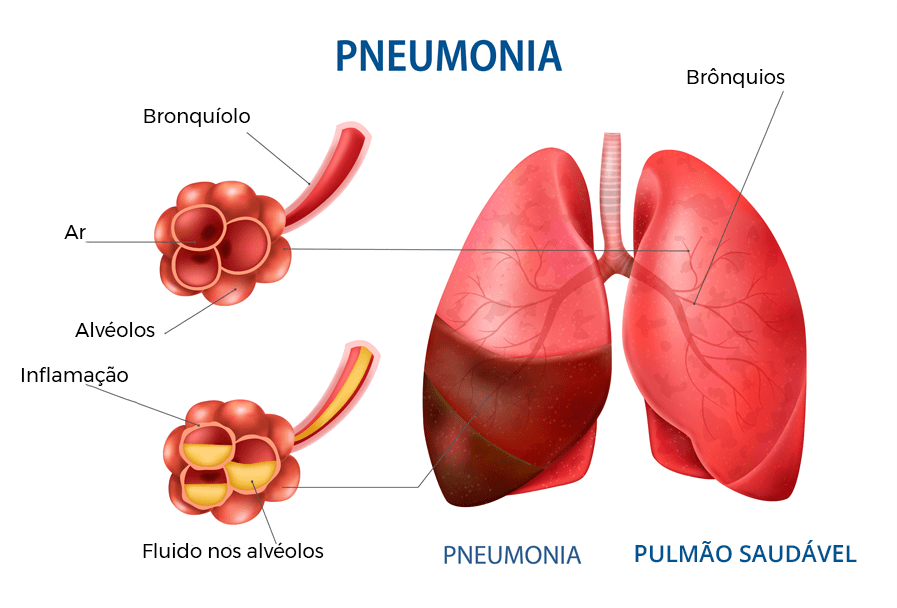
\includegraphics[width=300pt]{pictures/pneumonia -2.png}
    \caption{Pneumonia afetando um pulmão}
    \label{pic:pneumonia}
    \end{center}
\end{figure}

\begin{figure}[!ht]
    \begin{center}
    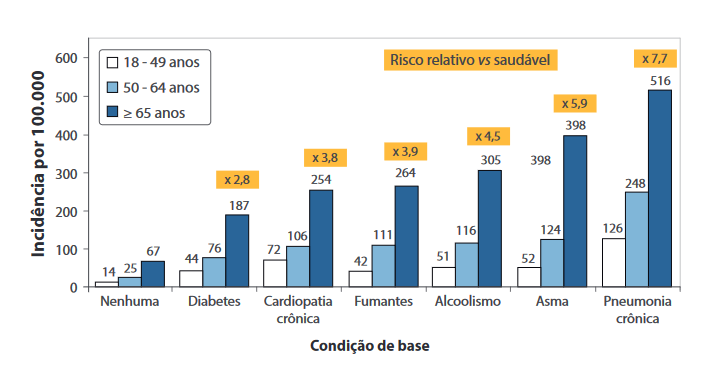
\includegraphics[width=350pt]{pictures/incidencia.png}
    \caption{Incidência de pneumonia em adultos }
    \label{pic:stats_pneumonia}
    \end{center}
\end{figure}




No Brasil, o Sistema Único de Saúde (SUS) registra anualmente mais de 600 mil internações por Pneumonia Adquirida na Comunidade (PAC) e Influenza. De janeiro a agosto de 2022, houve 44.523 mortes por pneumonia no país, um aumento significativo em relação ao mesmo período do ano anterior, que teve 31.027 óbitos. \cite{bvsmsDiaMundialPneumonia}

Em um contexto global, em 2019, a pneumonia foi responsável pela morte de cerca de 2,5 milhões de pessoas. Notavelmente, quase um terço dessas vítimas eram crianças com menos de 5 anos, fazendo da pneumonia a principal causa de morte para crianças nessa faixa etária . Apesar de ainda muitas crianças morrerem devido à pneumonia hoje, desde 1990 houve uma redução de mais de três vezes nas taxas de mortalidade infantil devido à doença em todo o mundo.\cite{OurWorldInDataPneumonia} Em 2019, a pneumonia resultou na morte de 740.180 crianças com menos de cinco anos, correspondendo a 14\% das mortes totais nessa faixa etária e a 22\% das mortes entre crianças de um a cinco anos, impactando famílias globalmente \cite{WHO2023Pneumonia}. 

A pneumonia bacteriana, que é a mais comum, é frequentemente causada pela bactéria \textit{Streptococcus pneumoniae}, embora outras bactérias como \textit{Mycoplasma pneumoniae} e \textit{Chlamydophila pneumoniae} também possam ser responsáveis. A pneumonia viral, por outro lado, é uma causa comum de pneumonia em crianças, com vírus respiratórios sendo os culpados frequentes. A pneumonia fúngica pode ocorrer em pessoas com sistemas imunológicos enfraquecidos \cite{WHO2023Pneumonia}.


Os sintomas da pneumonia podem variar, mas geralmente incluem tosse produtiva, febre, calafrios, fadiga, sudorese, dor no peito, confusão (em pessoas idosas) e falta de ar. O diagnóstico é geralmente feito com base nos sintomas e confirmado através de um exame físico, radiografia de tórax e, possivelmente, exames de sangue e culturas de escarro \cite{WHO2023Pneumonia}.

O tratamento para pneumonia depende da causa. A pneumonia bacteriana é geralmente tratada com antibióticos, enquanto a pneumonia viral pode ser tratada com antivirais. É também importante descansar, manter-se hidratado e tomar medicamentos para aliviar os sintomas. Para prevenção, existem vacinas como a vacina pneumocócica e a vacina contra a gripe, e medidas como lavar as mãos regularmente e evitar contato com pessoas doentes podem ser eficazes \cite{WHO2023Pneumonia}.

As complicações da pneumonia podem ser graves, podendo incluir infecção bacteriana no sangue (sepse), acúmulo de líquido e pus no espaço ao redor do pulmão (empema), e insuficiência respiratória. Indivíduos com sistemas imunológicos enfraquecidos, doenças crônicas, ou que estão em certos grupos etários (como crianças muito pequenas ou idosos) estão em maior risco de desenvolver pneumonia \cite{pneumoniaSymptoms}.  



\section{Redes Neurais}

Redes neurais é uma abordagem computacional ao processamento de informação, similiar ao sistema de nervoso dos seres humanos, especialmente o cérebro. Ela é uma sub-área de aprendizado de máquina, chamado de aprendizado profundo (\textit{deep learning}) capaz de realizar operações mais complexas e que necessitem de um poder computacional maior.

Sua unidade fundamental é chamada de neurônio, sendo apenas uma simplificação matemática do neurônio biológico. 

\begin{figure}[!ht]
    \begin{center}
    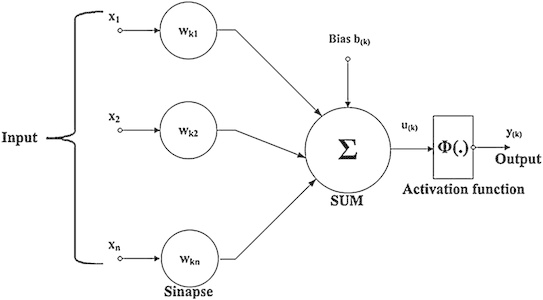
\includegraphics[width=350pt]{pictures/neuronio-matematico.png}
    \caption{Neurônio Matemático}
    \label{pic:neuronio}
    \end{center}
\end{figure}


Como ilustrado na figura \ref{pic:neuronio}, num primeiro momento, as informações são recebidas pelo neurônio em termos matemáticos (representados por $x_1, x_2, ... x_n$), ou seja, deve representar um valor numérico. Isso acontece porque, em uma rede neural, neurônios são conectados uns aos outros de maneira encadeada, por isso, é interessante manter esse padrão. Cada entrada de informação é associada à um peso. Esses pesos são valores númericos ajustáveis (indicados na imagem por $w_{k1}, w_{k2}, ...w_{kn}$ e representam a importância ou influência que uma determinada entrada pode impactar na saída do neurônio. Vale ressaltar que esses pesos inicialmente são definidos aleatoriamente e logo após ajustados durante o treinamento da rede \cite{GoodfellowBengioCourville2016}, \cite{Watt2016MachineLearning}.

\newpage

Recebendo essas entradas, o neurônio multiplica cada uma pelo seu respectivo peso e, em seguida, soma todos os produtos encontrados. Isso é chamado de função de soma, sendo representada na imagem pela letra grega ''$\sum$''. Normalmente esse processo de soma é representado matematicamente por um produto escalar, de um vetor de entradas $X$ por um vetor de pesos $W$.

$$
Soma = w_1 \times x_1 + w_2 \times x_2 + ... + w_n \times x_n
$$

Uma passo importante antes de calcular a soma ponderada é adicionar uma constante chamada de Viés (\textit{Bias}, representado como $b_{(k)}$ na imagem). O viés permite ajustar a saída do neurônio junto com os pesos, proporcionando um grau de liberdade adicional à rede neural. Podemos entender ele como uma maneira de ajustar a ''sensibilidade'' do neurônio. Após essa ''correção'' do viés, na soma ponderada, seu resultado é passado por uma função de ativação $\Phi(.)$, que introduz uma não-linearidade, permitindo que a rede neural modele operações mais complexas. As funções mais utilizadas são: \textbf{Sigmóide} (\ref{subfig:pictures/sigmoid.png}), \textbf{ReLU} (\ref{subfig:pictures/relu_func.png}), \textbf{Tangente Hiperbólica} (\ref{subfig:pictures/tanh.png}), \textbf{Softmax} (sendo frequentemente usada na camada de saída de problemas de classficação) e entre outros \cite{GoodfellowBengioCourville2016}, \cite{Watt2016MachineLearning}. 


\subimages{Funções de ativação}{45}
{
 \subimage[Sigmóide]{.35}{pictures/sigmoid.png}
 \subimage[ReLU]{.35}{pictures/relu_func.png}\\
 \subimage[Tangente Hiperbólica]{.35}{pictures/tanh.png} 
}


Por fim, o valor produzido pela função de ativação se torna a saída do neurônio. Como dito anteriormente, esse valor pode ser passado para outros neurônios, em sequência, ou até mesmo ser a saída definitiva da rede.

Para termos uma visão mais geral, podemos entender o processo de ativação da seguinte maneira:

\begin{enumerate}
    \item O neurônio recebe várias entradas
    \item Cada entrada é mutiplicada por seu respectivo peso
    \item Os produtos são somados junto ao \textit{Bias}
    \item A soma resultante passa por uma função de ativação para produzir a saída
\end{enumerate}

O objetivo do treinamento de uma rede neural é ajustar os pesos e vieses para que eles se adequem ao conjunto de dados fornecidos gerando uma saída muito próxima da desejada. Esses ajustes podem ser feitos utilizandos técnicas como o gradiente descente e a propagação reversa (\textit{backpropagation}) \cite{58337} \cite{Watt2016MachineLearning}.   



\section{Convolutional Neural Networks}

AS CNNs, também conhecidas como Redes Neurais Convolucionais, são uma categoria de redes neurais que se mostrou particularmente eficaz para tarefas de processamento de imagem. As CNNs são insipiradas pela visão biológica e foram projetadas para reconhecer padrões diretamente dos pixels de imagens com mínimo pré-processamento. A operação central das CNNs é a convolução. Ao invés de conectar totalmente todos os neurônios da camada anterior, um neurônio está conectado apenas a um pequeno patch localizado na camada anterior, através de um objeto matemático chamado de filtro ou \textit{kernel}. Um Kernel é uma matriz pequena, geralmente de tamanho $n \times n$, onde $n$ é um número ímpar como 3, 5 ou 7. Este kernel é ''deslizado'' ao longo da imagem para produzir um novo mapa de características.\cite{GoodfellowBengioCourville2016} Em cada ''deslizamento'' ocorre uma operação de convolução, que pode ser definida da seguinte maneira: 

Sejam $f(\tau)$ e $k(\tau)$ duas funções de domínio em $\mathbb{R}$, uma operação de convolução entre ambas pode ser escrita como:

$$
f \ast k = \int_{- \infty}^{\infty} f(\tau)k(t - \tau) \,dt 
$$

Numa camada convolucional, podemos generalizar a expressão de ''deslizamento'' do \textit{kernel} $k$ por uma imagem $I$ de tamanho $m \times n$, da seguinte forma:

$$
k \ast I = Z(i,j) = \sum_{m} \sum_{n}{k(m,n) I(i - m, j - n)}
$$

É importante ressaltar também que existem outras configurações que podemos alterar no \textit{kernel} para torná-lo mais preciso de modificável. Umas da alterações que podemos fazer é em relação a quantidade de pixels que ele se move de cada vez, ou melhor, a quantidade de pixels que é desconsiderada em cada turno. Essa disposição é chamada de \textit{stride} e está representada na imagem \ref{pic:stride} \cite{GoodfellowBengioCourville2016}. 


\begin{figure}[!ht]
    \begin{center}
    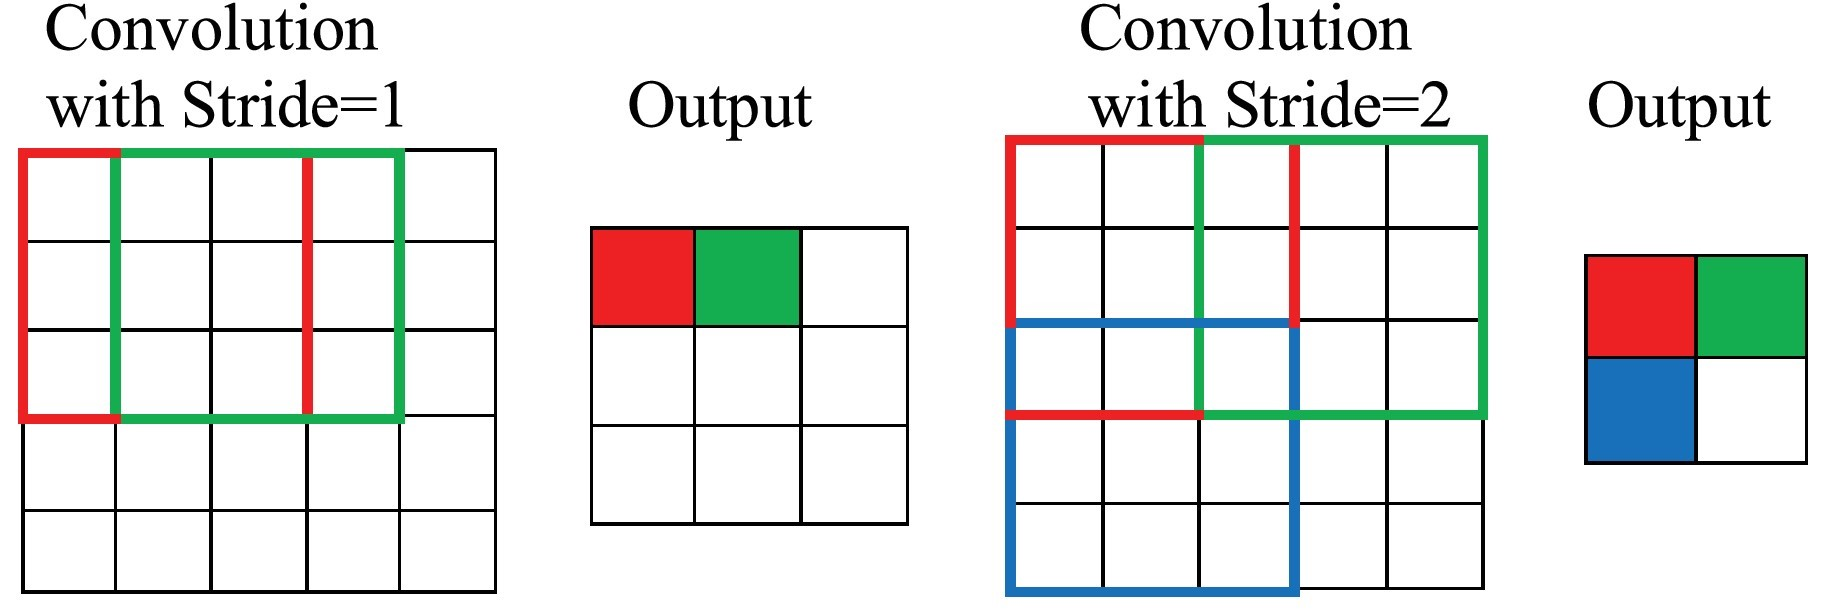
\includegraphics[width=350pt]{pictures/stride.jpg}
    \caption{Exemplo de stride}
    \label{pic:stride}
    \end{center}
\end{figure}


Outro conceito importante é o \textit{padding}, representado na imagem \ref{pic:padding}, que consiste em adicionar zeros ao entorno da imagem, ou do mapa de característica para controlar a dimensão espacial do resultado, usado frequentemente para manter a mesma dimensão espacial após a convolução \cite{GoodfellowBengioCourville2016}.


\begin{figure}[!ht]
    \begin{center}
    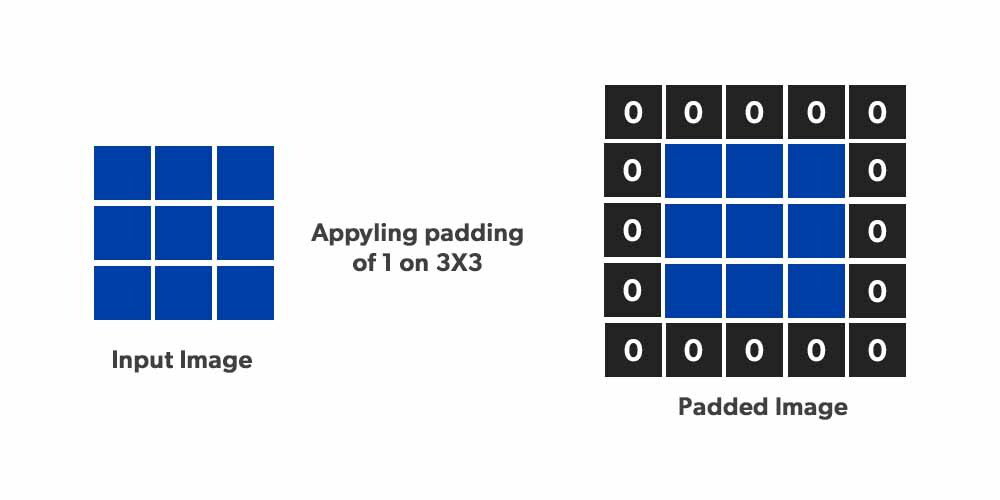
\includegraphics[width=350pt]{pictures/padding.jpg}
    \caption{Exemplo de padding}
    \label{pic:padding}
    \end{center}
\end{figure}


Um outro detalhe importante que precisa ser mencionado é sobre o canal de cores. Naturalmente, essa operações que foram descritas anteriormente são realizadas em apenas 1 dos canais da imagem, ou seja, se quisermos aplicar a metodologia apresentada, devemos repetir o processo para todos os canais \textbf{\textit{Red}}, \textbf{\textit{Green}} e \textbf{\textit{Blue}} \cite{Watt2016MachineLearning}.



Após passar pela camada convolucional, sua saída é passada por uma função de ativação, como mostrado na seção de \textbf{Redes Neurais}. Nesse caso, normalmente é utilizada a função ReLU (\textit{Rectified Linear Unit}) devido a sua eficácia \cite{Watt2016MachineLearning}.


\begin{figure}[!ht]
    \begin{center}
    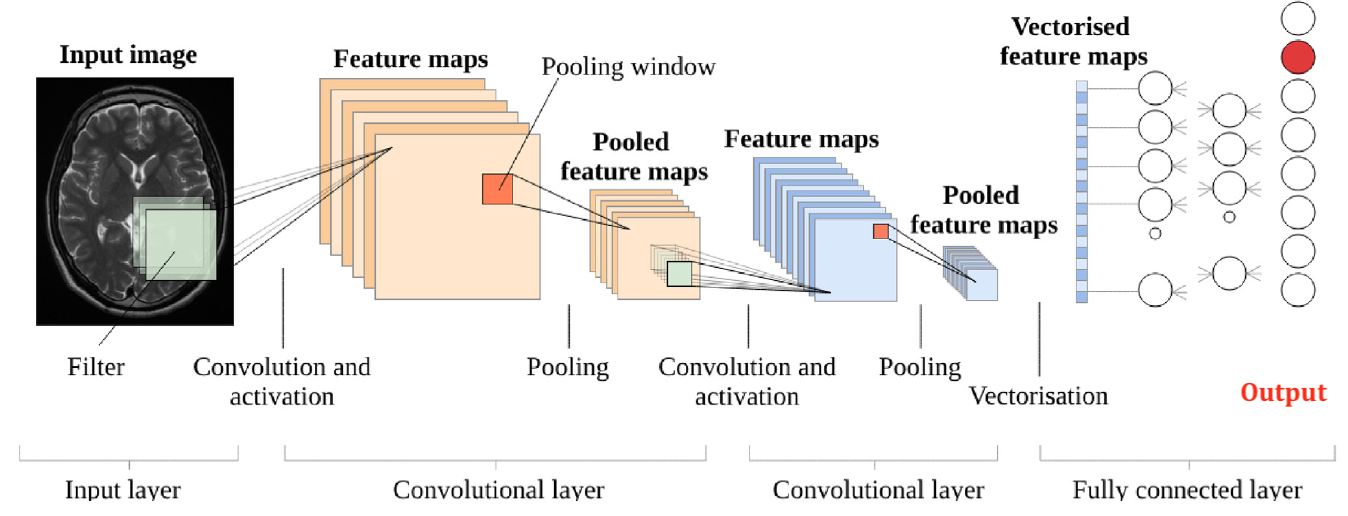
\includegraphics[width=350pt]{pictures/cnn_example_brain.png}
    \caption{\href{https://mriquestions.com/deep-network-types.html}{Visão completa de uma CNN}}
    \label{pic:cnn_complete}
    \end{center}
\end{figure}

Na imagem \ref{pic:cnn_complete} observamos todos os estágios para a criação de uma CNN, desde sua camada de \textit{input} até sua sáida. Percebemos também a presença de todas as camadas comentadas no texto, como as de convolução, \textit{polling} e a camada totalmente conectada.

\section{ResNet50}

A ResNet50 é uma variante da arquitetura de rede neural conhecida como Residual Network (ResNet), que foi uma das contribuições mais significativas no campo da visão computacional, particularmente no contexto de reconhecimento de imagens profundas. Desenvolvida por Kaiming He, Xiangyu Zhang, Shaoqing Ren e Jian Sun da Microsoft Research, estabelecendo um novo estado da arte para a classificação de imagens \cite{He2015}.

O principal problema que as conexões residuais visam resolver é o do "desaparecimento do gradiente", que é um desafio comum ao treinar redes neurais profundas. À medida que a rede se aprofunda, os gradientes (que são essenciais para a atualização dos pesos durante o treinamento) podem se tornar tão pequenos que não têm efeito perceptível, tornando a rede difícil ou impossível de treinar. As conexões residuais permitem que o sinal de gradiente seja diretamente propagado para camadas anteriores sem passar por todas as transformações de camadas intermediárias. Isso é feito adicionando a saída de uma camada anterior à saída de uma camada mais avançada, efetivamente permitindo que a rede aprenda a função de identidade se necessário. Isso significa que, em vez de aprender uma transformação direta, as camadas estão aprendendo um resíduo \cite{He2015}.

A ResNet50 é estruturada em quatro estágios principais, contendo uma série de blocos residuais, com o número de blocos em cada estágio sendo 3, 4, 6 e 3, respectivamente. À medida que a rede progride através dos estágios, o tamanho das características é reduzido e o número de filtros é aumentado para manter a carga computacional gerenciável \cite{Sharma2022Enhanced}.

Após todos os blocos residuais, a rede aplica uma camada de average pooling para condensar as características espaciais em um único vetor por característica. Isso é seguido por uma camada totalmente conectada que mapeia as características para o número desejado de classes e uma camada softmax para calcular as probabilidades de classificação \cite{Sharma2022Enhanced}.

Durante o treinamento, as conexões residuais facilitam a otimização da rede, mesmo com sua profundidade significativa. A ResNet50 pode ser treinada a partir do zero ou usada como uma rede pré-treinada em grandes conjuntos de dados, como o ImageNet, e ajustada para tarefas específicas através da transferência de aprendizado.


\begin{figure}[!ht]
    \begin{center}
    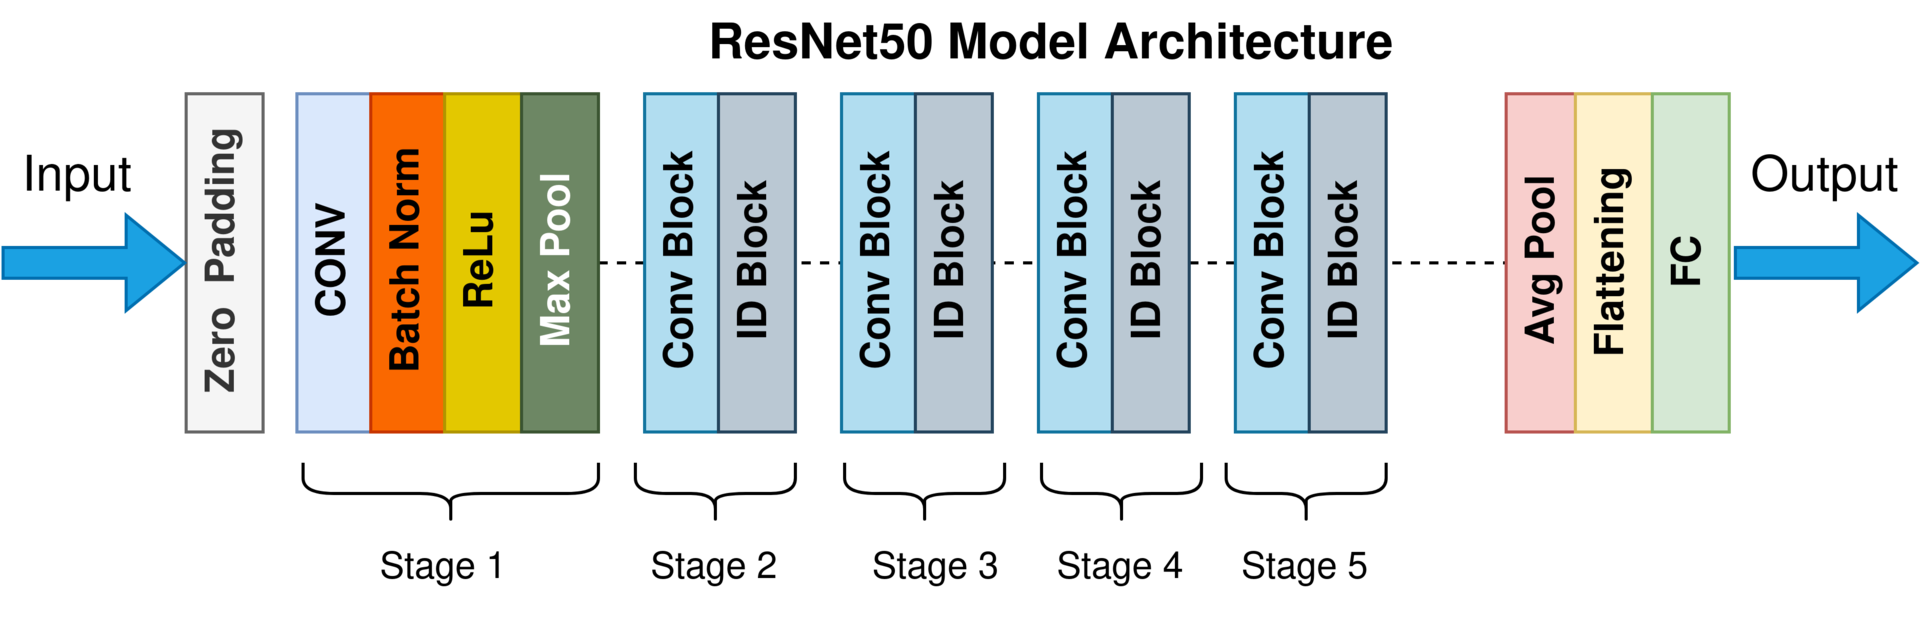
\includegraphics[width=350pt]{pictures/ResNet50.png}
    \caption{Arquitetura da ResNet50}
    \label{pic:resnet50}
    \end{center}
\end{figure}


Como representado na arquitetura da ResNet na imagem \ref{pic:resnet50}, a rede começa com uma única camada de convolução seguida por uma camada de max pooling, depois segue para uma série de blocos residuais e termina com uma camada de average pooling, uma camada totalmente conectada e uma função de ativação, como por exemplo a softmax, para tarefas de classificação.

A ResNet50, devido à sua profundidade e eficiência, tornou-se uma escolha popular para muitas aplicações de visão computacional, incluindo reconhecimento de objetos, detecção de objetos e segmentação semântica. Ela também é frequentemente usada como uma rede pré-treinada para transferência de aprendizado, onde uma rede treinada em um grande conjunto de dados (como o ImageNet) é adaptada para uma tarefa específica com um conjunto de dados menor \cite{Sharma2022Enhanced}.

O sucesso da ResNet e suas variantes inspirou muitas outras arquiteturas de redes neurais e continua a ser uma área ativa de pesquisa e aplicação. A capacidade de treinar redes profundas sem o problema do desaparecimento do gradiente abriu novas possibilidades para o design de arquiteturas de rede neural e ajudou a avançar o campo da inteligência artificial. Podemos entender mais até sobre o modelo e sua forma como foi construído no reposítório oficial da biblioteca TensorFlow, utilizada nessa tese, acesse \href{https://github.com/tensorflow/tpu/tree/master/models/experimental/resnet50_keras}{\textbf{Tensorflow: ResNet50}}


\section{InceptionV3}

Outro modelo de Rede Neural mundialmente utilizado é a InceptionV3. Ele foi introduzido pela primeira vez em 2014 por pesquisadores da Google na sua primeira versão (InceptionV1 ou GoogLeNet), após ter ganhado o desafio de classficação de imagem \textit{ImageNet Large Scale Visual Recognition Challenge} (\textbf{ILSVRC}) \cite{Szegedy2015RethinkingTI}. 

O modelo Inception v1 introduziu o conceito de módulos Inception. Eles foram criados com o objetivo de tornar as redes neurais convolucionais mais adaptáveis e capazes de extrair informações de uma vasta gama de entradas de imagem. A funcionalidade desses módulos se baseia em realizar várias operações de convolução simultaneamente, cada uma com filtros de tamanhos distintos, como 1x1, 3x3 e 5x5. Essa variedade permite que a rede detecte desde os detalhes mais sutis até as características mais amplas e abstratas das imagens. Em paralelo às convoluções, os módulos também executam operações de pooling, geralmente do tipo max pooling, que contribuem para a redução da dimensionalidade dos dados e ajudam a rede a se tornar invariante a pequenas mudanças e deslocamentos na imagem. Após realizar as convoluções e o pooling, a rede combina as saídas de todas essas operações paralelas, concatenando-as. Essa concatenação é feita ao longo do eixo do canal, garantindo que a riqueza de informações capturadas em cada processo seja mantida e transmitida adiante na rede \cite{7298594}.

Para evitar um crescimento exponencial no número de cálculos necessários, devido ao aumento das dimensões, os módulos Inception aplicam uma técnica de redução de dimensão. Isso é feito através do uso de convoluções 1x1 antes de aplicar filtros maiores, o que diminui a profundidade do volume de entrada sem perder informações essenciais. Com essa abordagem no modelo, podemos garatir que a rede neural mantenha sua eficiência computacional, mesmo enquanto processo grandes quantidades de dados \cite{7298594}.

Após as inovações da sua primeira versão, foi uma lançada uma V2 que trouxe uma melhoria na sua arquitetura original, incluindo otimizações para reduzir mais ainda o consumo operacional. Uma das melhorias inseridas foi a adição da \textit{batch normalization}, que por consequência, acelerou o treinamento do modelo \cite{PapersWithCode_InceptionV2}.

 A Inception v3 trouxe avanços notáveis em relação às suas versões antecessoras, mantendo as otimizações da Inception v2 e adicionando novas melhorias. A arquitetura, como representada na imagem \ref{pic:inceptionv3}, refinou os módulos Inception com ajustes que padronizam os tamanhos dos filtros de convolução, resultando em uma redução substancial do número de operações computacionais necessárias. Além disso, a Inception v3 substituiu as convoluções de maior dimensão por uma sequência de duas convoluções de 3x3, diminuindo assim o número de parâmetros e o custo computacional envolvido \cite{Szegedy2016RethinkingTI}.

\begin{figure}[!ht]
    \begin{center}
    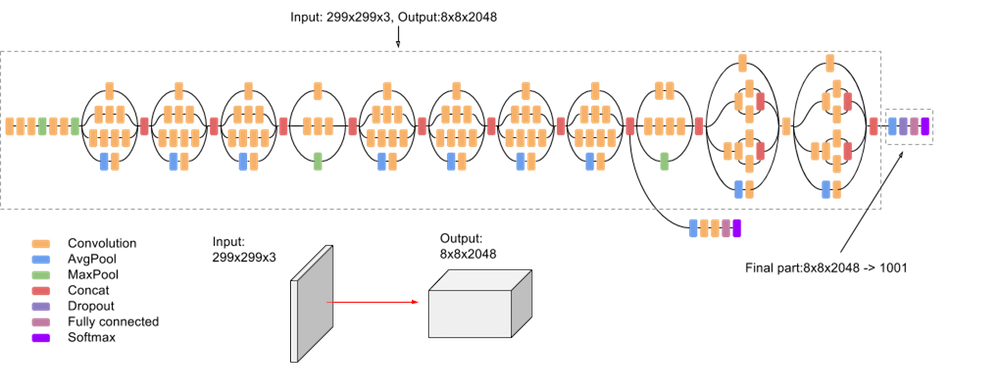
\includegraphics[width=350pt]{pictures/inception.png}
    \caption{Arquitetura da InceptionV3}
    \label{pic:inceptionv3}
    \end{center}
\end{figure}


Como citado anteriormente, a arquitetura também adotou o uso de convoluções assimétricas, empregando uma combinação de convoluções 1xN seguidas por Nx1, uma estratégia eficaz para substituir as convoluções quadradas tradicionais e reduzir ainda mais as demandas computacionais sem comprometer a eficiência na detecção de características. Para fortalecer a capacidade do modelo de generalizar a partir de conjuntos de dados de treinamento, a Inception v3 integrou técnicas de ampliação de dados mais avançadas, aumentando a robustez do modelo ao expô-lo a uma variedade mais ampla de variações de imagem durante o treinamento \cite{7298594}, \cite{Szegedy2016RethinkingTI}. Podemos entender mais até sobre o modelo e sua forma como foi construído no reposítório oficial da biblioteca TensorFlow, utilizada nessa tese, acesse \href{https://github.com/tensorflow/tpu/tree/master/models/experimental/inception}{\textbf{Tensorflow: Inception}}



\section{Otimizador RMSprop}

Algoritmos de otimização como desempenham um papel crucial no treinamento de redes neurais e outros modelos de aprendizado de máquina, pois aceleram a convergência para o mínimo da função de custo, o que é determinante para a avaliação do desempenho do modelo. Essa aceleração resulta em economia de tempo e recursos computacionais. Além disso, esses algoritmos previnem que o modelo fique retido em mínimos locais ou pontos de sela, garantindo assim que as soluções encontradas sejam robustas e representativas das melhores configurações possíveis \cite{Watt2016MachineLearning}. 

A capacidade de ajustar hiperparâmetros como a taxa de aprendizado é outra vantagem significativa, já que alguns algoritmos adaptam esses parâmetros dinamicamente durante o treinamento, potencialmente levando a resultados superiores. Eles são particularmente eficientes em grandes conjuntos de dados, onde calcular o gradiente para todos os exemplos é impraticável, optando por atualizar os parâmetros usando mini-lotes de dados \cite{Watt2016MachineLearning}.

A adaptabilidade desses algoritmos também permite que se ajustem a uma variedade de problemas, especialmente aqueles com superfícies de erro irregulares, suavizando as oscilações e promovendo atualizações mais consistentes. Eles mantêm a estabilidade numérica durante o treinamento, evitando extremos que poderiam resultar em problemas computacionais. Finalmente, ao otimizar a função de custo, contribuem para a capacidade de generalização do modelo, melhorando seu desempenho em dados novos e, portanto, sua utilidade em aplicações do mundo real \cite{Watt2016MachineLearning}.

Um dos algorítmos de otimização utilizado é o RMSProp, abreviação de "\textit{Root Mean Square Propagation}". Ele é um algoritmo de otimização projetado especificamente para treinar redes neurais artificiais (ANNs) e foi proposto por Geoff Hinton durante um curso online sobre Redes Neurais para Aprendizado de Máquina \cite{elshamy2023improving}.

Este algoritmo é uma adaptação do \textit{Stochastic Gradient Descent} (SGD) e faz parte dos métodos de taxa de aprendizagem adaptativa. O principal objetivo do RMSProp é ajustar de forma mais eficaz a taxa de aprendizagem durante o processo de treinamento. Para fazer isso, mantém uma média móvel (descontada) do quadrado dos gradientes e usa essa média para normalizar o gradiente ao atualizar os pesos da rede. Ou seja, ajusta a taxa de aprendizagem para cada parâmetro individualmente, em vez de ter uma taxa de aprendizagem fixa para todos os parâmetros \cite{elshamy2023improving}. Podemos escrever os cálculos de atualização da seguinte forma:

$$
E [g^2]_t = \beta E[g^2]_{t-1} + (1 - \beta)(\frac{\partial C}{\partial w})^2 
$$
$$
w_t = w_{t-1} - \frac{\eta}{\sqrt{E[g^2]_t}}\frac{\partial C}{ \partial w}
$$


Onde, $E[g]$ é a média móvel dos quadrados do gradientes, $\frac{\partial C}{\partial w}$ é o gradiente da função de custo com o respectivo peso ($w$); A constante $\eta$ é a taxa de aprendizado e $\beta$ é o parâmetro da média móvel, sendo normalmente utilizado como $0.9$ no seu valor.


\section{Otimizador Adam}

O otimizador Adam, abreviação de "\textit{Adaptive Moment Estimation}", é um algoritmo para otimização que é usado amplamente no treinamento de redes neurais e outras aplicações de aprendizado de máquina. Ele foi introduzido por Kingma e Ba em 2014 e é particularmente eficiente em casos com grandes volumes de dados e parâmetros, como mostram problemas envolvendo imagem \cite{Watt2016MachineLearning}.

Adam combina ideias do "\textit{momentum}" e do "RMSprop". No "\textit{momentum}", utiliza-se a média exponencialmente ponderada dos gradientes para acelerar o gradiente descendente. Esta técnica ajuda o algoritmo a acelerar em direções consistentes, o que auxilia na convergência mais rápida para mínimos. O RMSprop, por outro lado, adapta a taxa de aprendizado para cada parâmetro ao calcular uma média móvel exponencial dos quadrados dos gradientes. Isso permite ajustes mais finos do aprendizado, evitando passos demasiadamente grandes ou pequenos que poderiam prejudicar a convergência \cite{gess2023convergence}.

O otimizador Adam, portanto, herda as vantagens de ambos os métodos, oferecendo uma abordagem que consegue lidar bem com a variação nos gradientes e a escala dos dados. Isso é feito mantendo estimativas separadas dos primeiros momentos (o equivalente ao momentum) e dos segundos momentos (o equivalente ao RMSprop) dos gradientes \cite{gess2023convergence}.

O aspecto matemático do Adam envolve o cálculo das médias móveis exponencialmente ponderadas dos gradientes e dos quadrados dos gradientes. Entretanto, como essas médias são inicializadas como zero, o otimizador faz uma "correção de viés" para ajustar e escalar as médias móveis, garantindo que elas sejam imparciais. Intuitivamente, o Adam ajusta a descida do gradiente após cada iteração para mantê-la sob controle e imparcial durante todo o processo de otimização \cite{Watt2016MachineLearning}.

Em termos de desempenho, o Adam é conhecido por superar muitos outros otimizadores, proporcionando um treinamento eficiente e eficaz, com menor custo computacional e melhor desempenho em muitos cenários. O ajuste fino que o Adam proporciona, ao controlar a taxa de aprendizado de maneira adaptativa, permite que ele navegue eficientemente através de paisagens complexas de otimização, alcançando bons mínimos em tempo hábil e com estabilidade \cite{gess2023convergence}.


\begin{figure}[!ht]
    \begin{center}
    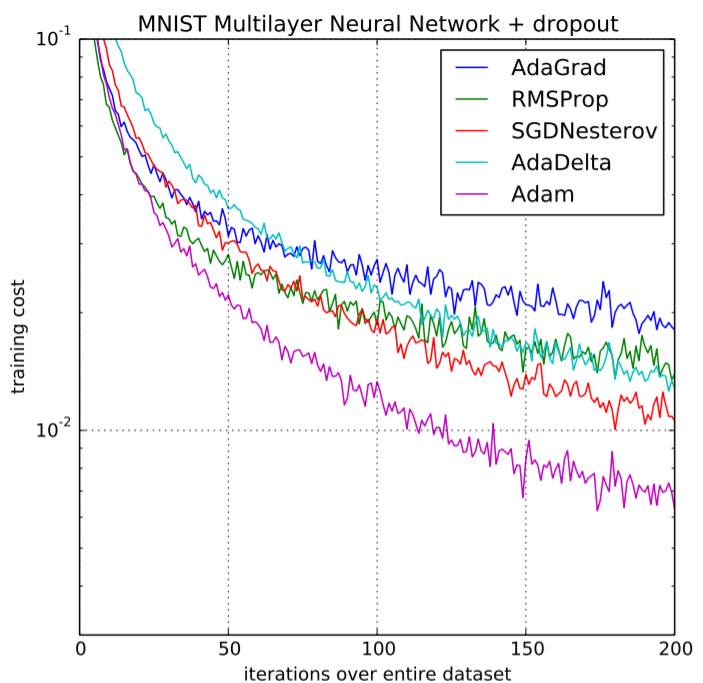
\includegraphics[width=250pt]{pictures/performance.png}
    \caption{Performance entre otimizadores}
    \label{pic:performance}
    \end{center}
\end{figure}


A imagem \ref{pic:performance}, mostra um comparativo entre diversos otimizadores aplicados à tarefa de classificar imagens do conjunto de dados \textbf{MNIST}, torna-se evidente que, apesar de todos visarem a minimização do erro, o Adam sobressai significativamente em termos de desempenho ao longo das iterações. Em contrapartida, o RMSProp, mencionado previamente, exibe um desempenho consistente, mas não extraordinário, situando-se em um patamar intermediário em relação aos demais otimizadores analisados.



%https://mriquestions.com/deep-network-types.html

  \chapter{Projeto e Especificação do Sistema}
\label{cha:Projeto e Especificação do Sistema}

Nesse capítulo serão abordadas mais informações sobre as bibliotecas necessárias para criação e treinamento dos modelos, detalhando cada uma de suas funções e métodos utilizados. Será apresentado também uma descrição detalhada do dataset utilizado para o treinamento como também seus metadados.

\section{Bibliotecas}

Para a confecção do projeto, foram utilizadas uma série de bibliotecas para a criação, teste, otimização e avaliação dos modelos de rede neural. 

\lstinputlisting[label=process,title={Bibliotecas utilizadas},caption={Bibliotecas utilizadas},language=Python]{codes/imports.py}

Primeiramente, \textbf{Matplotlib} e \textbf{Seaborn} são usadas para criar gráficos e visualizações. \textbf{Matplotlib} é a escolha tradicional para gráficos estáticos e interativos, enquanto Seaborn oferece uma abordagem mais estilizada para visualizações de dados.

O \textbf{Keras}, operando em cima da biblioteca \textbf{TensorFlow}, é uma API de alto nível para construir e treinar modelos de aprendizado profundo. Com essa biblioteca, é possível empilhar camadas de redes neurais usando o modelo \verb|Sequential| e adicionar uma variedade de camadas como \verb|Dense| para conexões densas, \verb|Conv2D| para convolução em dados de imagem, \verb|MaxPool2D| para pooling, \verb|Flatten| para achatar as dimensões dos dados, \verb|Dropout| para reduzir o overfitting e \verb|BatchNormalization| para normalizar as ativações dos neurônios. O \verb|ImageDataGenerator| é uma ferramenta poderosa para aumentar o conjunto de dados de imagem e melhorar o desempenho do modelo. Além disso, o \verb|ReduceLROnPlateau| é um callback que ajusta a taxa de aprendizado durante o treinamento para otimizar o processo.

O pacote \textbf{Scikit-learn} foi empregado para dividir o conjunto de dados em treino e teste com \verb|train_test_split| e avaliar o desempenho do modelo com métricas como \verb|classification_report| e \verb|confusion_matrix|, além de fornecer uma visualização clara do desempenho com \verb|ConfusionMatrixDisplay|. Vale ressaltar que a versão utilizada do pacote (2.1) ainda não possuia o método ConfusionMatrixDisplay, foi usado o pandas alido com o seaborn para fazer tal visualização.

É importante dizer que o \textbf{TensorFlow} é a base sobre a qual o Keras é construído, e o \textit{backend} do \textbf{Keras} permite operações de baixo nível que são independentes da plataforma, o que significa que é possível escrever código que é compatível com diferentes frameworks de aprendizado de máquina.

O \textbf{OpenCV} é uma biblioteca robusta para processamento de imagens e visão computacional, que permite manipular e processar imagens para tarefas como reconhecimento facial ou detecção de objetos, nesse caso, aplicado para leitura e carregamento dos conjuntos de dados. O módulo \textbf{os} foi utilizado para interagir com o sistema de arquivos do sistema operacional, permitindo operações como a leitura e escrita de arquivos.

Juntas, essas bibliotecas e funções formam um ecossistema completo para o desenvolvimento de projetos de aprendizado de máquina, desde a preparação e visualização de dados até a construção, treinamento e avaliação de modelos complexos, nesse caso, relacionados ao processamento de imagens médicas.


\section{Análise do Dataset}


Esta tese apresenta redes neurais projetadas para determinar a presença de pneumonia a partir de radiografias torácicas. Essas imagens de raio-X (anterior-posterior) foram selecionadas de retrospectivas de pacientes pediátricos de um a cinco anos de idade do Centro Médico de Mulheres e Crianças de Guangzhou, China, sendo todas elas parte de um atendimento clínico de rotina.

Para a análise das imagens de raio-X, todas as radiografias foram inicialmente examinadas para controle de qualidade, removendo todas as varreduras de baixa qualidade. Os diagnósticos para as imagens foram então classificados por dois médicos especialistas antes de serem liberados para treinar o sistema de IA. A fim de levar em conta quaisquer erros de classificação, o conjunto de avaliação também foi verificado por um terceiro especialista. 

O conjunto de dados usado para treinar e testar essas redes pode ser obtido no Kaggle sob o nome \href{https://www.kaggle.com/datasets/paultimothymooney/chest-xray-pneumonia/data}{"\textbf{Chest X-Ray Images (Pneumonia)}"}, ou no próprio artigo onde utilizaram esse dataset \cite{Kermany2018}. No total existem 5866 imagens, que estão divididas em três diretórios distintos:

\begin{enumerate}
    \item \textit{\textbf{test}}: Representando o conjunto de dados para testagem do modelo após ter sido treinado, contendo 234 imagens de pulmões saudáveis e 390 com pneumonia. 

    \item \textit{\textbf{train}}: Representando o conjunto de imagens que serão utilizadas para o treinamento do modelo, contendo 1351 imagens de pulmões saudáveis e 3875 imagens de pulmões que contrairam a doença.

    \item \textit{\textbf{val}}: Representando as imagens que serão utilizadas durante o treinamento do modelo, não para ajustar os pesos do modelo, e sim para servir como uma espécie de validação das previsões, monitorando a aprendizagem e generalização do modelo, ajudando a indentificar problemas como overfitting. Nesse caso um volume menor de imagens, com 8 de cada categoria.
    
\end{enumerate}


É importante ressaltar também que as imagens encontradas nessa base estão no formato \verb|.jpeg|, na escala de cores cinza e elas não possuem um tamanho fixo.
  \chapter{Implementação e Avaliação}
\label{cha:Implementação e Avaliação}


Nesse capítulo serão abordados todas as etapas da processamento, criação/treinamento e avaliação dos 3 modelos selecionados. Na etapa de treinamento será explicado um pouco do processamento das imagens, na fase criação/treinamento será exemplificado melhor o padrão de construção dos modelos e, por fim, na fase de avaliação serão exibidos os resultados encontrados.

\section{Análise e Processamento dos Dados}

Como apontado no capítulo \ref{cha:Projeto e Especificação do Sistema}, o dataset consiste numa série de imagens de raio-X de pulmões. As imagens têm extensão \verb|.jpeg|, não possuem um tamanho fixo e estão separadas em 3 pastas (\verb|train|, \verb|test| e \verb|val|) de acordo com suas devidas funções. Por isso, antes de começar o treinamento e avaliação dos modelos de rede neural, foi necessário passar por uma etapa de processamento, onde realizaremos transformações no conjunto de dados, seguindo o algorítmo \ref{alg:processamentoDados}.

\begin{algorithm}
    \DontPrintSemicolon
    \KwIn{Caminho de dados}
    \KwOut{Vetor com dados carregados}
    \BlankLine
    \emph{resultado $\xleftarrow{}$ cria\_lista\_vazia()}\;
    \ForAll{classe} {
        \emph{caminho $\xleftarrow{}$ monta\_caminho(Caminho de dados, classe)}\;
        \emph{acessa\_caminho(caminho)}\;
        \ForAll{imagem}{
            \emph{carrega\_imagem()}\;
            \emph{redimensiona\_imagem()}\;
            \emph{atualiza\_vetor(resultado, [imagem, classe])}\;
        }
    }
    \emph{Retorna resultado}\;
    
    \caption{Processamento dos dados}
    \label{alg:processamentoDados}
\end{algorithm}\DecMargin{1em}

O algorítmo \ref{alg:processamentoDados} recebe de entrada um diretório onde ele deverá ler as imagens e retorna um vetor com as imagens carregadas. Esse algorítmo será executado para todos os 3 diretórios (\verb|train|, \verb|test| e \verb|val|), onde ele percorrerá por todas as imagens redimensionando para o tamanho ideal (nesse caso sendo 150 pixels por 150 pixels). Por fim ele atualiza o vetor de saída com um novo vetor contendo a imagem transformada e sua classe (NORMAL ou PNEUMONIA).

Utilizando a função criada, podemos carregar as imagens para 3 cenários diferentes (\verb|train|, \verb|test| e \verb|val|) e analiser o conjunto. Um exemplo de imagens lidas aplicando a paleta de cores \verb|bone| está representada na imagen \ref{pic:3x3_raiox}.

\begin{figure}[!ht]
    \begin{center}
    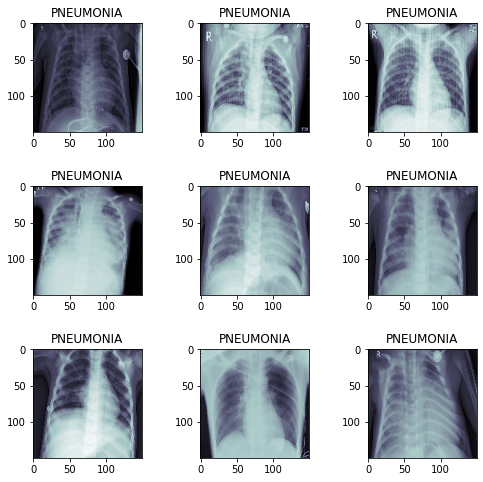
\includegraphics[width=350pt]{pictures/images_chest.png}
    \caption{Raio-X de pulmões}
    \label{pic:3x3_raiox}
    \end{center}
\end{figure}

Colocando as imagens em um dataframe da bilbioteca pandas, conseguimos ter uma visualização melhor e exibir gráficos envolvendo a quantidade de cada classe em cada estágio do processo. 

Na imagem \ref{pic:estagios_treinamento}, é trivial perceber que as classes  estão desbalanceadas no conjunto de dados, onde a barra vermelha representa as imagens de pulmões com pneumonia e a barra azul de pulmões saudáveis, tendo seus estágios de treino, teste e validação representando 89\%, 10\% e  0.2\% da base respectivamente. Sendo assim, será necessário aplicar uma etapa de enriquecimento de dados (\textit{data augmentation}) para gerar novas amostras para cada estágio.

\begin{figure}[!ht]
    \begin{center}
    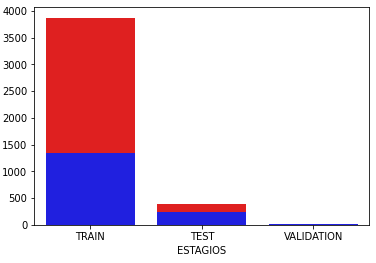
\includegraphics[width=300pt]{pictures/dados_estagios.png}
    \caption{Dados dos estágios}
    \label{pic:estagios_treinamento}
    \end{center}
\end{figure}

\newpage
Para seguir com o passo do enriquecimento de dados, utilizamos uma função da biblioteca \verb|keras| chamada de \verb|ImageDataGenerator| que aceita uma série de parâmetros para gerar diferentes variações nas imagens. Para o treinamento e validação do modelo foram utilizados diferentes configurações:

\begin{enumerate}
    \item As imagens foram rotacionadas em 30º, sendo útil para reconhecer objetos que podem aparecer em várias orientações.
    \item As imagens foram transladadas ligeiramente para cima e para lado em 10\% do seu valor, com o objetivo de reconhecer traços de pneumonia mesmo não estando centralizado na imagem
    \item Um zoom de 20\% foi aplicado tendo como finalidade reconhecer objetos de diferentes escalas.
    \item Um \textit{flip} horizontal, já que a orientação horizontal do raio-X não importa. Nesse caso, não tem problema trocar pulmões esquerdos por direitos, pois o objetivo do modelo é puramente binário.
\end{enumerate}

Outra alteração necessária a ser feita foi a normalização dos valores dos pixels. Nas imagens atuais, os valores de cores estão entre 1 e 255, porém um modelo de CNN performa melhor se essa grandeza estiver entre 0 e 1. 
\newpage 

\section{Criação dos Modelos}

Uma função específica foi desenvolvida para construir e treinar modelos seguindo um formato padrão. Utiliza-se a função Sequential da biblioteca keras para definir o modelo, sobre a qual são empilhadas diversas camadas necessárias. Estas podem incluir convoluções, operações de \textit{pooling}, normalizações, entre outras. Todas as funções empregadas na criação dos modelos aderem a este padrão estabelecido exemplificado no algorítmo \ref{alg:criacaoModelo}


\begin{algorithm}
\DontPrintSemicolon
\KwIn{Número de épocas, tamanho do lote, dados de treino e dados de validação}
\KwOut{Histórico de treinamento e modelo treinado}
\BlankLine
\emph{modelo $\xleftarrow{}$ Sequential}\;
\emph{modelo.empilha\_camadas\_necessárias()}\;
\emph{modelo.compilar(otimizador=otimizador\_escolhido)}\;
\emph{histórico $\xleftarrow{}$ modelo.treinar(dados de treino, dados de validação, número de epocas, tamanho do lote)}\;
\emph{Retorna histórico, modelo}
\caption{Criação e treinamento de um modelo}\label{alg:criacaoModelo}
\end{algorithm}\DecMargin{1em}

Como especificado na \ref{cha:Pesquisas Realizadas}, os algorítmos de rede neural ResNet50 e InceptionV3, foram treinados com imagens com 3 canais de cores. No caso do \textit{dataset} utilizado, não será necessário aplicar técnica alguma para "colorir" as imagens de escala cinza, basta apenas repetir a mesma camada cinza 3 vezes ao enviar as imagens para o modelo. 


\section{Resultados}

Depois de treinar os modelos, avaliamos sua eficácia usando várias métricas, incluindo acurácia, perda durante as fases de treinamento e teste, matrizes de confusão e relatórios de classificação. Experimentos variados foram realizados, empregando otimizadores como \textbf{Adam} e \textbf{RMSProp} em combinação com modelos como InceptionV3, ResNet50, e uma rede neural convolucional. Os treinamentos foram realizados com 20 épocas, gerando os resultados encontrados na tabela \ref{tab:resultados_tabela}.
\newpage

\begin{table}[!h]
    \centering
    \renewcommand{\arraystretch}{1.5} % Aumenta o espaçamento entre as linhas
    \begin{tabular}{c|c|c|c|c|c|c|c}
       Modelo  & Otimizador & Precisão & Perda & Acurácia & f1-score & Recall & Miss \\
         \hline  
        CNN & RMSProp & 0.88 & 0.54 & 87.82\% & 0.88 & 0.88 & 76 \\
        ResNet50 & RMSProp & 0.91 & 0.23 & 90.86\% & 0.91 & 0.91 & 57\\ 
        InceptionV3 & RMSProp & 0.94 & 0.15 & 94.23 \% & 0.94 & 0.94 & 36 \\
        CNN & Adam & 0.89 & 0.27& 88.94\% &  0.89 &  0.89 & 69 \\
        ResNet50 & Adam & 0.93 & 0.17 & 93.42\% & 0.93 & 0.93 & 41 \\
        \cellcolor{green!25}InceptionV3 & \cellcolor{green!25}Adam & \cellcolor{green!25}0.95 &  \cellcolor{green!25}0.16 &  \cellcolor{green!25}95.19\% & \cellcolor{green!25}0.95 & \cellcolor{green!25}0.95 &  \cellcolor{green!25}30  
    \end{tabular}
    \caption{Resultados do treinamento}
    \label{tab:resultados_tabela}
\end{table}

A precisão é determinada pela proporção de predições acertadas para uma determinada classe em relação ao total de predições feitas para essa classe. Já o recall mede a proporção de predições acertadas para uma classe em comparação com o número total de casos verdadeiros dessa classe no conjunto de dados. O F1-Score, por sua vez, é calculado como a média harmônica da precisão e do recall, resultando em uma métrica única que balanceia as duas. Depois de calcular essas métricas para cada classe, realiza-se uma média delas para chegar aos valores apresentados na tabela.

Analisando mais detalhadamente a tabela \ref{tab:resultados_tabela} é perceptível que, quando foi feita a troca do otimizador RMSProp para Adam tivemos um aumento de até 2 pontos percentuais na acurácia, recall, f1-score e precisão, assim como a queda nesse caso, bem mais significativa, da perda. Ambos cenários indicam resultado positivos para esse dataset.

\begin{figure}[!ht]
    \begin{center}
    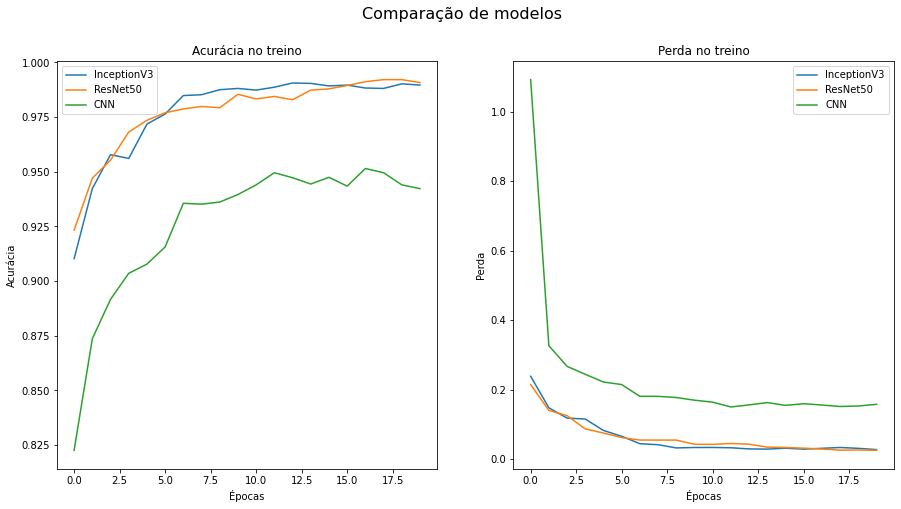
\includegraphics[width=400pt]{pictures/comparação entre modelos.png}
    \caption{Comparação de acurácia e perda}
    \label{pic:grafico_comparativo}
    \end{center}
\end{figure}

\newpage 

Analisando a imgem \ref{pic:grafico_comparativo}, percebemos que a curva da CNN se distancia das outras, mantendo uma acurácia menor e uma perda maior. Isso se dá devido ao nível de simplicidade e à ausência de pesos pré-treinados, como é o caso da InceptionV3 e da ResNet50. Falando um pouco sobre esses dois últimos modelos, é notável que ambos ficam muito próximos tanto no quesito de minimizar a perda quanto a maximizar a acurácia. De um modo geral, a rede neural InceptionV3 se sai melhor do que a ResNet50, pelo fato de convergir para seus valores ideais de maneira mais "rápida".

Analisando as matrizes de confusão para cada um dos modelos, são notados alguns resultados interessantes:

\begin{table}[!ht]
    \centering
    \begin{tabular}{l|l|c|c|c}
        \multicolumn{2}{c}{}&\multicolumn{2}{c}{Valor previsto}&\\
        \cline{3-4}
        \multicolumn{2}{c|}{}&Pneumonia&Normal&\multicolumn{1}{c}{Total}\\
        \cline{2-4}
        \multirow{2}{*}{Valor real}& Pneumonia & $356$ & $34$ & $390$\\
        \cline{2-4}
        & Normal & $35$ & $199$ & $234$\\
        \cline{2-4}
        \multicolumn{1}{c}{} & \multicolumn{1}{c}{Total} & \multicolumn{1}{c}{$391$} & \multicolumn{    1}{c}{$233$} & \multicolumn{1}{c}{$624$}\\
    \end{tabular}
    \caption{CNN - Matriz de confusão}
    \label{tab:cm_cnn}
\end{table}


Para os resultados previstos incorretamente, o pior caso, seriam os falsos positivos. Na CNN genérica montada eles representam aproximadamente 5.4\% do total de previsões, como mostra a tabela \ref{tab:cm_cnn}.

\newpage

\begin{table}[!ht]
    \centering
    \begin{tabular}{l|l|c|c|c}
        \multicolumn{2}{c}{}&\multicolumn{2}{c}{Valor previsto}&\\
        \cline{3-4}
        \multicolumn{2}{c|}{}&Pneumonia&Normal&\multicolumn{1}{c}{Total}\\
        \cline{2-4}
        \multirow{2}{*}{Valor real}& Pneumonia & $373$ & $17$ & $390$\\
        \cline{2-4}
        & Normal & $24$ & $210$ & $234$\\
        \cline{2-4}
        \multicolumn{1}{c}{} & \multicolumn{1}{c}{Total} & \multicolumn{1}{c}{$397$} & \multicolumn{    1}{c}{$227$} & \multicolumn{1}{c}{$624$}\\
    \end{tabular}
    \caption{ResNet50 - Matriz de confusão}
    \label{tab:res_cm}
\end{table}

Implementando um modelo mais robusto, é notória a diferença, representada na tabela \ref{tab:res_cm}, em ambos os casos incorretos com falsos positivos caindo 50\% e falsos negativos caindo 25\%.

\begin{table}[!ht]
    \centering
    \begin{tabular}{l|l|c|c|c}
        \multicolumn{2}{c}{}&\multicolumn{2}{c}{Valor previsto}&\\
        \cline{3-4}
        \multicolumn{2}{c|}{}&Pneumonia&Normal&\multicolumn{1}{c}{Total}\\
        \cline{2-4}
        \multirow{2}{*}{Valor real}& Pneumonia & $382$ & $8$ & $390$\\
        \cline{2-4}
        & Normal & $22$ & $212$ & $234$\\
        \cline{2-4}
        \multicolumn{1}{c}{} & \multicolumn{1}{c}{Total} & \multicolumn{1}{c}{$404$} & \multicolumn{    1}{c}{$220$} & \multicolumn{1}{c}{$624$}\\
    \end{tabular}
    \caption{InceptionV3 - Matriz de confusão}
    \label{tab:cm_incep}
\end{table}

Por fim, no InceptionV3 são encontrados os menores valores de classificações incorretas em todo o teste. Podemos ver na tabela \ref{tab:cm_incep} que, o total de falsos positivos decresceu 76\% em relação ao valor original, e os falsos negativos, um total de 37\%.

Com base no que foi apresentado, fica evidente que o modelo InceptionV3 supera os demais em eficácia, otimizando a precisão e reduzindo significativamente as perdas. Esse modelo se destaca especialmente na matriz de confusão ao registrar o menor número de falsos positivos e negativos. Essa característica é crucial, particularmente em análises médicas de doenças, onde um resultado falso negativo pode ter consequências graves para a saúde do paciente. Portanto, a eficiência do InceptionV3 em minimizar esses erros contribui diretamente para a confiabilidade e segurança dos diagnósticos.

  \chapter{Considerações Finais}
\label{cha:Considerações Finais}

Como lido anteriormente, a questão do uso de inteligência artificial aplicada na área de imagens médicas é um ganho positivo para profissionais de saúde. Existindo um modelo pré-treinado é possível: 

\begin{enumerate}
    \item  Melhorar a precisão do diagnóstico, podendo analisar imagens com padrões de doença sutis demais para detecção humana, como citada na introdução o caso da detecção do cancer de mama 5 anos antes de se formar completamente.
    \item Reduzir tempo de diagnósticos, analisando grandes volumes de dados de imagem rapidamente, tornado-se crucial para situações de emergência.
    \item Minimizar erros humanos que podem ocorrer devido á fadiga viés ou simplesmente limitações humanas na interpretação de imagens complexas.
\end{enumerate}

Com os modelos testados nessa tese, foi possível chegar à um resultado bem positivo de acurácia, mesmo tendo uma base de dados completamente enviesada para casos de pneumonia. O modelo que se mais destacou foi o \textbf{InceptionV3} aliado com o otimizador \textbf{Adam}, apresentando uma acurácia de 95.19\%, com pequenas incidências de erros.  

Para os próximos passos do projeto, seria possível treinar os modelos (CNN, ResNet50 e InceptionV3) em uma base balaceada entre as classes de pneumonia e saudável, gerando uma confiabilidade maior no modelo e por consequência diminuindo as ocorrências de falsos negativos nos resultados. Seria possível também, aplicar a mesma lógica de classificação à outros de tipos de casos como doenças oculares, cardíacas, ósseas/musculares e até mesmo para detecção de tumores.  

Embora os benefícios sejam consideráveis, substituir médicos e profissionais da saúde exclusivamente por inteligências artificiais não é viável. Isso ocorre porque, apesar da menor incidência de erros, esses modelos ainda são suscetíveis a equívocos ocasionais. Como ilustrado pelas matrizes de confusão no capítulo anterior, mesmo reduzindo ao máximo os casos de falsos negativos, houve 22 pacientes que correram o risco de receber um diagnóstico falso de não terem pneumonia, quando na verdade a possuíam. Erros desse tipo podem ameaçar a vida dos pacientes e de outros.

Dessa forma, é fundamental reconhecer o papel insubstituível da experiência humana e do julgamento clínico na área da saúde. A inteligência artificial deve ser vista como uma ferramenta poderosa que pode melhorar a eficiência e a precisão dos diagnósticos, mas sempre complementando e trabalhando em conjunto com as habilidades e conhecimentos dos profissionais de saúde. O equilíbrio entre tecnologia e atendimento humano é essencial para garantir uma assistência médica de alta qualidade, centrada no paciente e adaptada às complexidades e variabilidades inerentes ao campo da saúde. 



  %% ...
  \arial
  \bibliographystyle{abnt-alf} % \bibliographystyle{abnt-num}
  \bibliography{main} 
\end{document}

